\documentclass{article}
\usepackage{pythontex}
\usepackage{gensymb}
\usepackage{amssymb}
\usepackage{pgfkeys}
\usepackage{etoolbox}
\usepackage{ifthen}
\usepackage{graphicx}
\usepackage{listings}
\usepackage{xcolor}

%New colors defined below
\definecolor{codegreen}{rgb}{0,0.6,0}
\definecolor{codegray}{rgb}{0.5,0.5,0.5}
\definecolor{codepurple}{rgb}{0.58,0,0.82}
\definecolor{backcolour}{rgb}{0.95,0.95,0.92}

%Code listing style named "mystyle"
\lstdefinestyle{mystyle}{
  backgroundcolor=\color{backcolour},   commentstyle=\color{codegreen},
  keywordstyle=\color{magenta},
  numberstyle=\tiny\color{codegray},
  stringstyle=\color{codepurple},
  basicstyle=\ttfamily\footnotesize,
  breakatwhitespace=false,         
  breaklines=true,                 
  captionpos=b,                    
  keepspaces=true,                 
  numbers=left,                    
  numbersep=5pt,                  
  showspaces=false,                
  showstringspaces=false,
  showtabs=false,                  
  tabsize=2
}


%"mystyle" code listing set
\lstset{style=mystyle}

\begin{document}
\begin{center}


\rule{\textwidth}{1.6pt}\vspace*{-\baselineskip}\vspace*{2pt} % Thick horizontal line
\rule{\textwidth}{0.4pt}\\[\baselineskip] % Thin horizontal line

{\LARGE Determine Refractive Index of Material \\[0.2\baselineskip] of a prism using Sodium Source}% Title

\rule{\textwidth}{0.4pt}\vspace*{-\baselineskip}\vspace{3.2pt} % Thin horizontal line
\rule{\textwidth}{1.6pt}\\[2\baselineskip] % Thick horizontal line




\textbf{\Large \\[\baselineskip] SGTB Khalsa College, University of Delhi}\\[\baselineskip]
\textbf{\Large Preetpal Singh(2020PHY1140) \\[\baselineskip] Anjali(2020PHY1164)}\\[\baselineskip] 

\vspace*{\baselineskip}
\textbf{\Large Unique Paper Code: 32221202}\\[\baselineskip] 
\vspace*{\baselineskip}
 
\textbf{\Large Paper Title: Waves and Optics Lab}\\[\baselineskip] 
\vspace*{\baselineskip}
\textbf{\Large Submitted on: June 4, 2021}\\[\baselineskip] 
\vspace*{\baselineskip}
\textbf{\Large Due On: June 6, 2021}\\[\baselineskip] 
\vspace*{\baselineskip}
\textbf{\Large File Name: 1140\_Mamta\_A1c}\\[\baselineskip]
\vspace*{\baselineskip}
\textbf{\Large B.Sc(H) Physics Sem II}\\[\baselineskip] 
\vspace*{\baselineskip}
\vspace*{\baselineskip}
\textbf{\Large Submitted to: Dr. Mamta}\\[\baselineskip] 


\end{center}
\newpage
\begin{pycode}
import pandas as pd
data = pd.read_csv('data1.csv')
	
\end{pycode}
\section{\LARGE AIM}
\Large
To Determine Refractive Index of Material of a prism using Sodium Source
\section{\LARGE APPARATUS}
Spectrometer, prism, prism clamp, sodium vapour lamp, lens. etc.
\section{\LARGE PROCEDURE}
\begin{itemize}
    \item Focus Telescope on distant object.
    \item When focus is correct, start button is activated. Then click Start button.
    \item Switch on the light by clicking Switch On Light button.
    \item Focus the slit using Slit focus slider.
    \item Bring Vernier to 0 degree and 180 degree position using Vernier Table Slider.
    \item Place the prism.
    \item Bring telescope using Telescope Slider to a position of (180 - 2i) degree by rotating it in anti-clockwise direction, where (i) is the angle of incidence.
    \item Move Vernier Table in clockwise direction to coincide slit with cross wire.
    \item Now move telescope in clockwise direction so that refracted ray goes in it and coincide slit with cross wire. 
    \item Note down reading for both Verniers .This will be reading for refracted Ray. 
    \item Remove the Prism.
    \item Move telescope in anti-clockwise direction to get direct ray in it and coincide slit with cross wire. 
    \item Note down the readings for both Verniers now as well. This will be reading for Direct Ray.
\end{itemize}

\section{\LARGE PRECAUTIONS}
\begin{itemize}
    \item Slit should be as narrow as possible. 
    \item Vernier numbering should remain fixed throughout the experiment.
    \item Prism position should be maintained properly.
    \item Fine adjustment of telescope must be used in each case.
    
\end{itemize}
\newpage
\section{\LARGE OBSERVATIONS}
\subsection{\Large Least Count of Spectrometer} 

$27 MSD = 30 VSD$
\vspace*{\baselineskip}
\newline
 $1 VSD$ = $\frac{27}{30}$MSD
 \vspace*{\baselineskip}
\newline
Least count = $1 MSD - 1 VSD$
\vspace*{\baselineskip}
\newline
$1 MSD$ - $\frac{27}{30}$$MSD$ = $\frac{3}{30}$MSD
\vspace*{\baselineskip}

\newline
\vspace*{\baselineskip}
On main scale 20 divisions = 10$\degree$
\vspace*{\baselineskip}
\newline
1 division = $(1/2)\degree$ = 1 MSD
\vspace*{\baselineskip}
\newline 
\therefore L.C = (\frac{3}{30}) \times (\frac{1}{2})\degree = (\frac{1}{20})\degree
\vspace*{\baselineskip}
\newline


= $(\frac{1}{20} \times 60)'$ = $3'$

\subsection{\Large Angle of Deviation}
\begin{tabular}{cccccc}
\hline $\angle i^{\circ}$ & $vs$ & $\angle r^{\circ}$ & $\angle d^{\circ}$ & $(\angle r^{\circ}-\angle d^{\circ})$ & $\angle mean^{\circ}$ \\
\hline
$30 ^{\circ}$ & $V1$ & $42 ^{\circ} \ 30'$ & $89 ^{\circ} \ 30'$ & $47 ^{\circ}$ &  $47 ^{\circ}$  \\ 

 & $V2$ & $222 ^{\circ} \ 30'$ & $269 ^{\circ} \ 30'$ & $47 ^{\circ}$ &  \\

$35 ^{\circ}$ & $V1$ & $53 ^{\circ} \ 30'$ & $94 ^{\circ} \ 30'$ & $41 ^{\circ}$ & $41 ^{\circ}$ \\

 & $V2$ & $233 ^{\circ} \ 30'$ & $274 ^{\circ} \ 30'$ & $41 ^{\circ}$ &  \\

$40 ^{\circ}$ & $V1$ & $61 ^{\circ}$ & $99 ^{\circ} \ 30'$ & $38 ^{\circ} \ 30'$ & $38 ^{\circ} \ 30'$ \\

 & $V2$ & $241 ^{\circ}$ & $279 ^{\circ} \ 30'$ & $38 ^{\circ} \ 30'$ &  \\

$45 ^{\circ}$ & $V1$ & $67 ^{\circ}$ & $104 ^{\circ} \ 30'$ & $37 ^{\circ} \ 30'$ &  $37 ^{\circ} \ 30'$\\

 & $V2$ & $247 ^{\circ}$ & $284 ^{\circ} \ 30'$ & $37 ^{\circ}$ &  \\

$50 ^{\circ}$ & $V1$ & $72 ^{\circ} \ 30'$ & $109 ^{\circ} \ 30'$ & $37 ^{\circ}$ &  $37 ^{\circ} \ 15'$\\

 & $V2$ & $252 ^{\circ}$ & $289 ^{\circ} \ 30'$ & $37 ^{\circ} \ 30'$ &  \\

$55 ^{\circ}$ & $V1$ & $77 ^{\circ}$ & $114 ^{\circ} \ 30'$ & $37 ^{\circ} \ 30'$ &  $37 ^{\circ} \ 30'$\\

 & $V2$ & $257 ^{\circ}$ & $294 ^{\circ} \ 30'$ & $37 ^{\circ} \ 30'$ &  \\

$60 ^{\circ}$ & $V1$ & $80 ^{\circ} \ 30'$ & $119 ^{\circ} \ 30'$ & $39 ^{\circ} \ 30'$ &  $39 ^{\circ}$\\

 & $V2$ & $260 ^{\circ} \ 30'$ & $299 ^{\circ} \ 30'$ & $39 ^{\circ}$ &  \\


\hline
\end{tabular}
\subsubsection{Take observation for angle of deviation for various angles of incidence i}

\begin{pycode}
  
 
import matplotlib.pyplot as plt
from scipy.optimize import curve_fit
import numpy as np

def rad(x):
    return (x * np.pi/180)

def func(i,A,n):
    return i - A + np.arcsin(n * np.sin(A - np.arcsin(np.sin(i)/n)))

def min_dev(y_cal,xlim):
    list = []
    for j in range(len(y_cal)):
        xlim[j]
        if y_cal[j] == np.min(y_cal):
            list.append(xlim[j])
            list.append(np.min(y_cal))
    mini = np.array(list)
    print("\nCoordinates of minima of the graph (x,y):\n",mini)
    print("\n Angle of minimum deviation from Graph is: ",min(y_cal))
    return mini


if __name__ == "__main__":
    datax = np.array([30,35,40,45,50,55,60])
    mean_dev_deg = np.array([47,41,38,37,37,37,39])
    mean_dev_min = np.array([0,0,30,30,15,30,0])
    datay= np.array((mean_dev_deg) + (mean_dev_min/60))
    xlim = np.linspace(30,60,100)

    popt, pcov = curve_fit(func,rad(datax),rad(datay))
    print("\nAngle of prism and Refractive index of the prism from fitting:\n",popt,"\n")
    y_cal = np.array(func(rad(xlim),*popt)) * 180/np.pi
    print(y_cal)
    mini = min_dev(y_cal,xlim)

    plt.style.use("ggplot")
    plt.title("Graph between $\delta$ vs i")
    plt.xlabel('Angle of incidence (i)')
    plt.ylabel('Angle of deviation ($\delta$)')
    plt.scatter(datax,datay,color = "b",label = "Experimental data")
    plt.scatter(mini[0],mini[1],c = "g",label = "Minimum deviation point")
    plt.plot(xlim,np.array(func(rad(xlim),*popt) * 180/np.pi), color = "r",label = "Fitting curve")
    plt.legend()
    plt.show()
\end{pycode}

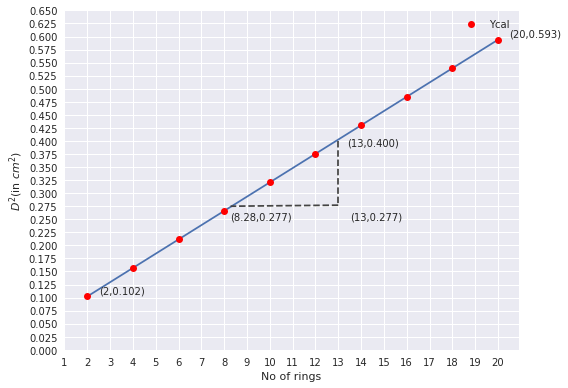
\includegraphics[width = 12cm, height = 12cm]{Figure.png}




\section{RESULT AND DISCUSSION}
{\Large ️Minimum angle of deviation is 37\degree11'45''}
\begin{itemize}
    \item We just went through the theory of experiment by sharing links with info of concerned points and definitions.
    \item We just worked together on simulator by sharing screen via Gmeet.
    \item We evaluated the readings taken.
    \item We discussed the error part.
\end{itemize}

\section{Contribution of Team Mates}
\begin{description}
		\item[Anjali : ] She did most of the theoretical part including working on simulator.
		\item[Preetpal Singh : ] He did Python programming and Latex part. 
	\end{description}
	
	
	
\section{\LARGE Programming Code}
\begin{lstlisting}[language=Python]
import matplotlib.pyplot as plt
from scipy.optimize import curve_fit
import numpy as np

def rad(x):
    return (x * np.pi/180)

def func(i,A,n):
    return i - A + np.arcsin(n * np.sin(A - np.arcsin(np.sin(i)/n)))

def min_dev(y_cal,xlim):
    list = []
    for j in range(len(y_cal)):
        xlim[j]
        if y_cal[j] == np.min(y_cal):
            list.append(xlim[j])
            list.append(np.min(y_cal))
    mini = np.array(list)
    print("\nCoordinates of minima of the graph (x,y):\n",mini)
    print("\n Angle of minimum deviation from Graph is: ",min(y_cal))
    return mini
    

if __name__ == "__main__":
    datax = np.array([30,35,40,45,50,55,60])
    mean_dev_deg = np.array([47,41,38,37,37,37,39])
    mean_dev_min = np.array([0,0,30,30,15,30,0])
    datay= np.array((mean_dev_deg) + (mean_dev_min/60))
    xlim = np.linspace(30,60,100)

    popt, pcov = curve_fit(func,rad(datax),rad(datay))
    print("\nAngle of prism and Refractive index of the prism from fitting:\n",popt,"\n")
    y_cal = np.array(func(rad(xlim),*popt)) * 180/np.pi
    print(y_cal)
    mini = min_dev(y_cal,xlim)
    
    plt.style.use("ggplot")
    plt.title("Graph between $\delta$ vs i")
    plt.xlabel('Angle of incidence (i)')
    plt.ylabel('Angle of deviation ($\delta$)')
    plt.scatter(datax,datay,color = "b",label = "Experimental data")
    plt.scatter(mini[0],mini[1],c = "g",label = "Minimum deviation point")
    plt.plot(xlim,np.array(func(rad(xlim),*popt) * 180/np.pi), color = "r",label = "Fitting curve")
    plt.legend()
    plt.show()
\end{lstlisting}
\newpage
\section{\Large References}
    \url{https://vlab.amrita.edu/}

\end{document}
